% Options for packages loaded elsewhere
\PassOptionsToPackage{unicode}{hyperref}
\PassOptionsToPackage{hyphens}{url}
%
\documentclass[
]{article}
\usepackage{amsmath,amssymb}
\usepackage{lmodern}
\usepackage{iftex}
\ifPDFTeX
  \usepackage[T1]{fontenc}
  \usepackage[utf8]{inputenc}
  \usepackage{textcomp} % provide euro and other symbols
\else % if luatex or xetex
  \usepackage{unicode-math}
  \defaultfontfeatures{Scale=MatchLowercase}
  \defaultfontfeatures[\rmfamily]{Ligatures=TeX,Scale=1}
\fi
% Use upquote if available, for straight quotes in verbatim environments
\IfFileExists{upquote.sty}{\usepackage{upquote}}{}
\IfFileExists{microtype.sty}{% use microtype if available
  \usepackage[]{microtype}
  \UseMicrotypeSet[protrusion]{basicmath} % disable protrusion for tt fonts
}{}
\makeatletter
\@ifundefined{KOMAClassName}{% if non-KOMA class
  \IfFileExists{parskip.sty}{%
    \usepackage{parskip}
  }{% else
    \setlength{\parindent}{0pt}
    \setlength{\parskip}{6pt plus 2pt minus 1pt}}
}{% if KOMA class
  \KOMAoptions{parskip=half}}
\makeatother
\usepackage{xcolor}
\usepackage[margin=2cm]{geometry}
\usepackage{color}
\usepackage{fancyvrb}
\newcommand{\VerbBar}{|}
\newcommand{\VERB}{\Verb[commandchars=\\\{\}]}
\DefineVerbatimEnvironment{Highlighting}{Verbatim}{commandchars=\\\{\}}
% Add ',fontsize=\small' for more characters per line
\usepackage{framed}
\definecolor{shadecolor}{RGB}{248,248,248}
\newenvironment{Shaded}{\begin{snugshade}}{\end{snugshade}}
\newcommand{\AlertTok}[1]{\textcolor[rgb]{0.94,0.16,0.16}{#1}}
\newcommand{\AnnotationTok}[1]{\textcolor[rgb]{0.56,0.35,0.01}{\textbf{\textit{#1}}}}
\newcommand{\AttributeTok}[1]{\textcolor[rgb]{0.77,0.63,0.00}{#1}}
\newcommand{\BaseNTok}[1]{\textcolor[rgb]{0.00,0.00,0.81}{#1}}
\newcommand{\BuiltInTok}[1]{#1}
\newcommand{\CharTok}[1]{\textcolor[rgb]{0.31,0.60,0.02}{#1}}
\newcommand{\CommentTok}[1]{\textcolor[rgb]{0.56,0.35,0.01}{\textit{#1}}}
\newcommand{\CommentVarTok}[1]{\textcolor[rgb]{0.56,0.35,0.01}{\textbf{\textit{#1}}}}
\newcommand{\ConstantTok}[1]{\textcolor[rgb]{0.00,0.00,0.00}{#1}}
\newcommand{\ControlFlowTok}[1]{\textcolor[rgb]{0.13,0.29,0.53}{\textbf{#1}}}
\newcommand{\DataTypeTok}[1]{\textcolor[rgb]{0.13,0.29,0.53}{#1}}
\newcommand{\DecValTok}[1]{\textcolor[rgb]{0.00,0.00,0.81}{#1}}
\newcommand{\DocumentationTok}[1]{\textcolor[rgb]{0.56,0.35,0.01}{\textbf{\textit{#1}}}}
\newcommand{\ErrorTok}[1]{\textcolor[rgb]{0.64,0.00,0.00}{\textbf{#1}}}
\newcommand{\ExtensionTok}[1]{#1}
\newcommand{\FloatTok}[1]{\textcolor[rgb]{0.00,0.00,0.81}{#1}}
\newcommand{\FunctionTok}[1]{\textcolor[rgb]{0.00,0.00,0.00}{#1}}
\newcommand{\ImportTok}[1]{#1}
\newcommand{\InformationTok}[1]{\textcolor[rgb]{0.56,0.35,0.01}{\textbf{\textit{#1}}}}
\newcommand{\KeywordTok}[1]{\textcolor[rgb]{0.13,0.29,0.53}{\textbf{#1}}}
\newcommand{\NormalTok}[1]{#1}
\newcommand{\OperatorTok}[1]{\textcolor[rgb]{0.81,0.36,0.00}{\textbf{#1}}}
\newcommand{\OtherTok}[1]{\textcolor[rgb]{0.56,0.35,0.01}{#1}}
\newcommand{\PreprocessorTok}[1]{\textcolor[rgb]{0.56,0.35,0.01}{\textit{#1}}}
\newcommand{\RegionMarkerTok}[1]{#1}
\newcommand{\SpecialCharTok}[1]{\textcolor[rgb]{0.00,0.00,0.00}{#1}}
\newcommand{\SpecialStringTok}[1]{\textcolor[rgb]{0.31,0.60,0.02}{#1}}
\newcommand{\StringTok}[1]{\textcolor[rgb]{0.31,0.60,0.02}{#1}}
\newcommand{\VariableTok}[1]{\textcolor[rgb]{0.00,0.00,0.00}{#1}}
\newcommand{\VerbatimStringTok}[1]{\textcolor[rgb]{0.31,0.60,0.02}{#1}}
\newcommand{\WarningTok}[1]{\textcolor[rgb]{0.56,0.35,0.01}{\textbf{\textit{#1}}}}
\usepackage{longtable,booktabs,array}
\usepackage{calc} % for calculating minipage widths
% Correct order of tables after \paragraph or \subparagraph
\usepackage{etoolbox}
\makeatletter
\patchcmd\longtable{\par}{\if@noskipsec\mbox{}\fi\par}{}{}
\makeatother
% Allow footnotes in longtable head/foot
\IfFileExists{footnotehyper.sty}{\usepackage{footnotehyper}}{\usepackage{footnote}}
\makesavenoteenv{longtable}
\usepackage{graphicx}
\makeatletter
\def\maxwidth{\ifdim\Gin@nat@width>\linewidth\linewidth\else\Gin@nat@width\fi}
\def\maxheight{\ifdim\Gin@nat@height>\textheight\textheight\else\Gin@nat@height\fi}
\makeatother
% Scale images if necessary, so that they will not overflow the page
% margins by default, and it is still possible to overwrite the defaults
% using explicit options in \includegraphics[width, height, ...]{}
\setkeys{Gin}{width=\maxwidth,height=\maxheight,keepaspectratio}
% Set default figure placement to htbp
\makeatletter
\def\fps@figure{htbp}
\makeatother
\setlength{\emergencystretch}{3em} % prevent overfull lines
\providecommand{\tightlist}{%
  \setlength{\itemsep}{0pt}\setlength{\parskip}{0pt}}
\setcounter{secnumdepth}{-\maxdimen} % remove section numbering
\ifLuaTeX
  \usepackage{selnolig}  % disable illegal ligatures
\fi
\IfFileExists{bookmark.sty}{\usepackage{bookmark}}{\usepackage{hyperref}}
\IfFileExists{xurl.sty}{\usepackage{xurl}}{} % add URL line breaks if available
\urlstyle{same} % disable monospaced font for URLs
\hypersetup{
  pdftitle={STAT 679 / 992 Midterm},
  hidelinks,
  pdfcreator={LaTeX via pandoc}}

\title{STAT 679 / 992 Midterm}
\author{}
\date{\vspace{-2.5em}}

\begin{document}
\maketitle

\begin{itemize}
\tightlist
\item
  This exam lasts from 11:00 - 12:15pm on October 24, 2022. There are 7
  questions.
\item
  This exam is closed notes and closed computer.
\item
  You may use a 1-page cheat sheet (8.5 x 11in or A4 size). You may use
  both sides, but the cheat sheet must be handwritten.
\item
  If you need extra space, you may write on the back of the page. Please
  indicate somewhere that your answer continues.
\item
  The instructors will only be able to answer clarifying questions
  during the exam. They will be sitting at the back of the room.
\end{itemize}

\begin{longtable}[]{@{}lllllllll@{}}
\toprule()
Question & Q1 & Q2 & Q3 & Q4 & Q5 & Q6 & Q7 & Total \\
\midrule()
\endhead
Score & & & & & & & & \\
Possible & 2 & 2 & 4 & 5 & 5 & 6 & 6 & 30 \\
\bottomrule()
\end{longtable}

\hypertarget{q1}{%
\subsubsection{Q1}\label{q1}}

Circle whether the following statements about interactive visualization
with Shiny are TRUE or FALSE.

\begin{enumerate}
\def\labelenumi{\alph{enumi}.}
\item
  TRUE FALSE The \texttt{bs\_theme()} function from the \texttt{bslib}
  library can be used to both customize the overall UI theme and modify
  fonts in a Shiny application.
\item
  TRUE FALSE In order to implement a brush graphical query that only
  moves in the \texttt{x} direction, a version of the following code
  will have to appear at some point within the application's server
  function,

\begin{Shaded}
\begin{Highlighting}[]
\FunctionTok{plotOutput}\NormalTok{(}\StringTok{"output\_id"}\NormalTok{, }\AttributeTok{brush =} \FunctionTok{brushOpts}\NormalTok{(}\StringTok{"plot\_brush"}\NormalTok{, }\AttributeTok{direction =} \StringTok{"x"}\NormalTok{))}\ErrorTok{)}
\end{Highlighting}
\end{Shaded}
\item
  TRUE FALSE By using a \texttt{reactive(\{...\})} expression within a
  server function, it is possible to reduce the number of edges
  appearing in an application's reactive graph.
\item
  TRUE FALSE If the code

\begin{Shaded}
\begin{Highlighting}[]
\NormalTok{output}\SpecialCharTok{$}\NormalTok{scatterplot }\OtherTok{\textless{}{-}} \FunctionTok{renderPlot}\NormalTok{(\{}
  \FunctionTok{ggplot}\NormalTok{(}\FunctionTok{filter}\NormalTok{(df, group }\SpecialCharTok{\%in\%}\NormalTok{ input}\SpecialCharTok{$}\NormalTok{groups)) }\SpecialCharTok{+}
    \FunctionTok{geom\_point}\NormalTok{(}\FunctionTok{aes}\NormalTok{(x, y))}
\NormalTok{\})}
\end{Highlighting}
\end{Shaded}

  appeared in an application's server, then we would expect to see
  \texttt{plotOutput(input\$scatterplot)} in the UI.
\end{enumerate}

\hypertarget{q2}{%
\subsubsection{Q2}\label{q2}}

Circle whether the following statements about interactive visualization
with Shiny are TRUE or FALSE.

\begin{enumerate}
\def\labelenumi{\alph{enumi}.}
\item
  TRUE FALSE Imagine that we want to highlight a subset of circles that
  have been given the class name ``highlighted.'' The code below could
  be used to increase the radius of all circles within this class to 5
  pixels.

\begin{Shaded}
\begin{Highlighting}[]
\FunctionTok{d3.selectAll}\NormalTok{(}\StringTok{"\#highlighted"}\NormalTok{)}
  \FunctionTok{.attr}\NormalTok{(}\StringTok{"r"}\NormalTok{, }\DecValTok{5}\NormalTok{)}
\end{Highlighting}
\end{Shaded}
\item
  TRUE FALSE Imagine that \texttt{circle\_data} is an array of objects
  giving x and y coordinates in fields called \texttt{x} and \texttt{y}.
  The code below will append one circle for each object in the array at
  the \texttt{x} and \texttt{y} pixel coordinates of the SVG.

\begin{Shaded}
\begin{Highlighting}[]
\FunctionTok{d3.data}\NormalTok{(circle\_data)}\FunctionTok{.enter}\NormalTok{()}
  \FunctionTok{.append}\NormalTok{(}\StringTok{"circle"}\NormalTok{)}
  \FunctionTok{.attrs}\NormalTok{(\{}
\NormalTok{    cx}\SpecialCharTok{:}\NormalTok{ d }\SpecialCharTok{=\textgreater{}}\NormalTok{ d.x,}
\NormalTok{    cy}\SpecialCharTok{:}\NormalTok{ d }\SpecialCharTok{=\textgreater{}}\NormalTok{ d.y,}
\NormalTok{    r}\SpecialCharTok{:} \DecValTok{5}
\NormalTok{  \})}
\end{Highlighting}
\end{Shaded}
\item
  TRUE FALSE Imagine that our visualization of the \texttt{circle\_data}
  array currently displays 10 circles arranged from left to right. The
  code below will reduce the size of the three circles furthest to the
  right before completely removing their corresponding HTML tags from
  the page.

\begin{Shaded}
\begin{Highlighting}[]
\NormalTok{circles }\OtherTok{=} \FunctionTok{circles.slice}\NormalTok{(}\DecValTok{3}\NormalTok{)}
\FunctionTok{d3.select}\NormalTok{(}\StringTok{"svg"}\NormalTok{)}
  \FunctionTok{.selectAll}\NormalTok{(}\StringTok{"circle"}\NormalTok{)}
  \FunctionTok{.data}\NormalTok{(circle\_data)}\FunctionTok{.exit}\NormalTok{()}
  \FunctionTok{.transition}\NormalTok{()}
  \FunctionTok{.duration}\NormalTok{(}\DecValTok{4000}\NormalTok{)}
  \FunctionTok{.attr}\NormalTok{(}\StringTok{"r"}\NormalTok{, }\DecValTok{0}\NormalTok{)}
  \FunctionTok{.remove}\NormalTok{()}
\end{Highlighting}
\end{Shaded}
\item
  TRUE FALSE ID functions can be supplied to the second of argument a
  \texttt{.data()} call in order to associate each appended HTML element
  with a property appearing in the underlying array element.
\end{enumerate}

\hypertarget{q3}{%
\subsubsection{Q3}\label{q3}}

The example visualization below comes from the course notes. It is
supposed to help readers compare country populations.

\begin{Shaded}
\begin{Highlighting}[]
\FunctionTok{library}\NormalTok{(tidyverse)}
\NormalTok{gapminder }\OtherTok{\textless{}{-}} \FunctionTok{read\_csv}\NormalTok{(}\StringTok{"https://uwmadison.box.com/shared/static/dyz0qohqvgake2ghm4ngupbltkzpqb7t.csv"}\NormalTok{, }\AttributeTok{col\_types =} \FunctionTok{cols}\NormalTok{()) }\SpecialCharTok{\%\textgreater{}\%} 
  \FunctionTok{mutate}\NormalTok{(}\AttributeTok{cluster =} \FunctionTok{as.factor}\NormalTok{(cluster))}

\FunctionTok{print}\NormalTok{(}\FunctionTok{head}\NormalTok{(gapminder, }\DecValTok{3}\NormalTok{))}
\end{Highlighting}
\end{Shaded}

\begin{verbatim}
## # A tibble: 3 x 6
##    year country     cluster      pop life_expect fertility
##   <dbl> <chr>       <fct>      <dbl>       <dbl>     <dbl>
## 1  1955 Afghanistan 0        8891209        30.3       7.7
## 2  1960 Afghanistan 0        9829450        32.0       7.7
## 3  1965 Afghanistan 0       10997885        34.0       7.7
\end{verbatim}

\begin{Shaded}
\begin{Highlighting}[]
\FunctionTok{ggplot}\NormalTok{(}\FunctionTok{filter}\NormalTok{(gapminder, year }\SpecialCharTok{==} \DecValTok{2000}\NormalTok{)) }\SpecialCharTok{+}
 \FunctionTok{geom\_col}\NormalTok{(}\FunctionTok{aes}\NormalTok{(country, pop))}
\end{Highlighting}
\end{Shaded}

\begin{center}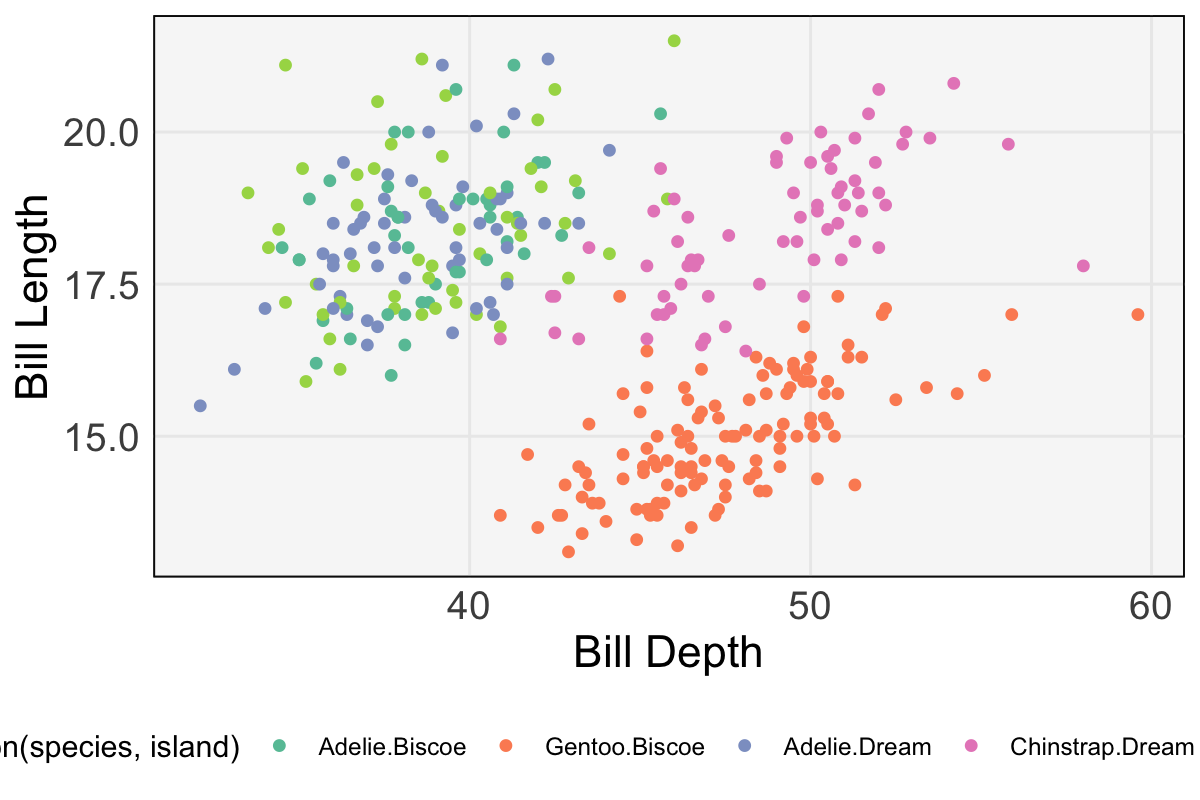
\includegraphics[width=200px]{midterm1_files/figure-latex/unnamed-chunk-7-1} \end{center}

\begin{enumerate}
\def\labelenumi{\alph{enumi}.}
\item
  (2 points) Give two distinct examples of specific user queries related
  to the overall \texttt{gapminder} dataset printed above that are
  difficult (or impossible) to make with the current display.

  \[\\[2.5cm]\]
\item
  (2 points) Sketch an alternative \texttt{ggplot2} implementation that
  addresses the issues you raised in part (a). Why does it help?

  \[\\[2.5cm]\]
\end{enumerate}

\hypertarget{q4}{%
\subsubsection{Q4}\label{q4}}

This problem asks you to share your conceptual and practical
understanding of D3 scales.

\begin{enumerate}
\def\labelenumi{\alph{enumi}.}
\tightlist
\item
  (2 points) In your own words, what purpose do D3 scales serve?
\end{enumerate}

\[\\[2.5cm]\]

\begin{enumerate}
\def\labelenumi{\alph{enumi}.}
\setcounter{enumi}{1}
\tightlist
\item
  (2 points) The figure below visualizes miles per gallon vs.~horsepower
  for a cars in an array called \texttt{cars}. Define a D3 scale that
  could be used to set the \texttt{x} coordinates of each circle on the
  SVG canvas. Assume that the SVG is 600 pixels tall and 1000 pixels
  wide. For reference, each car's data object has a form like
  \texttt{\{name:\ "chevrolet\ chevelle\ malibu",\ mpg:\ 18,\ horsepower:\ 130\}}.
\end{enumerate}

\begin{flushleft}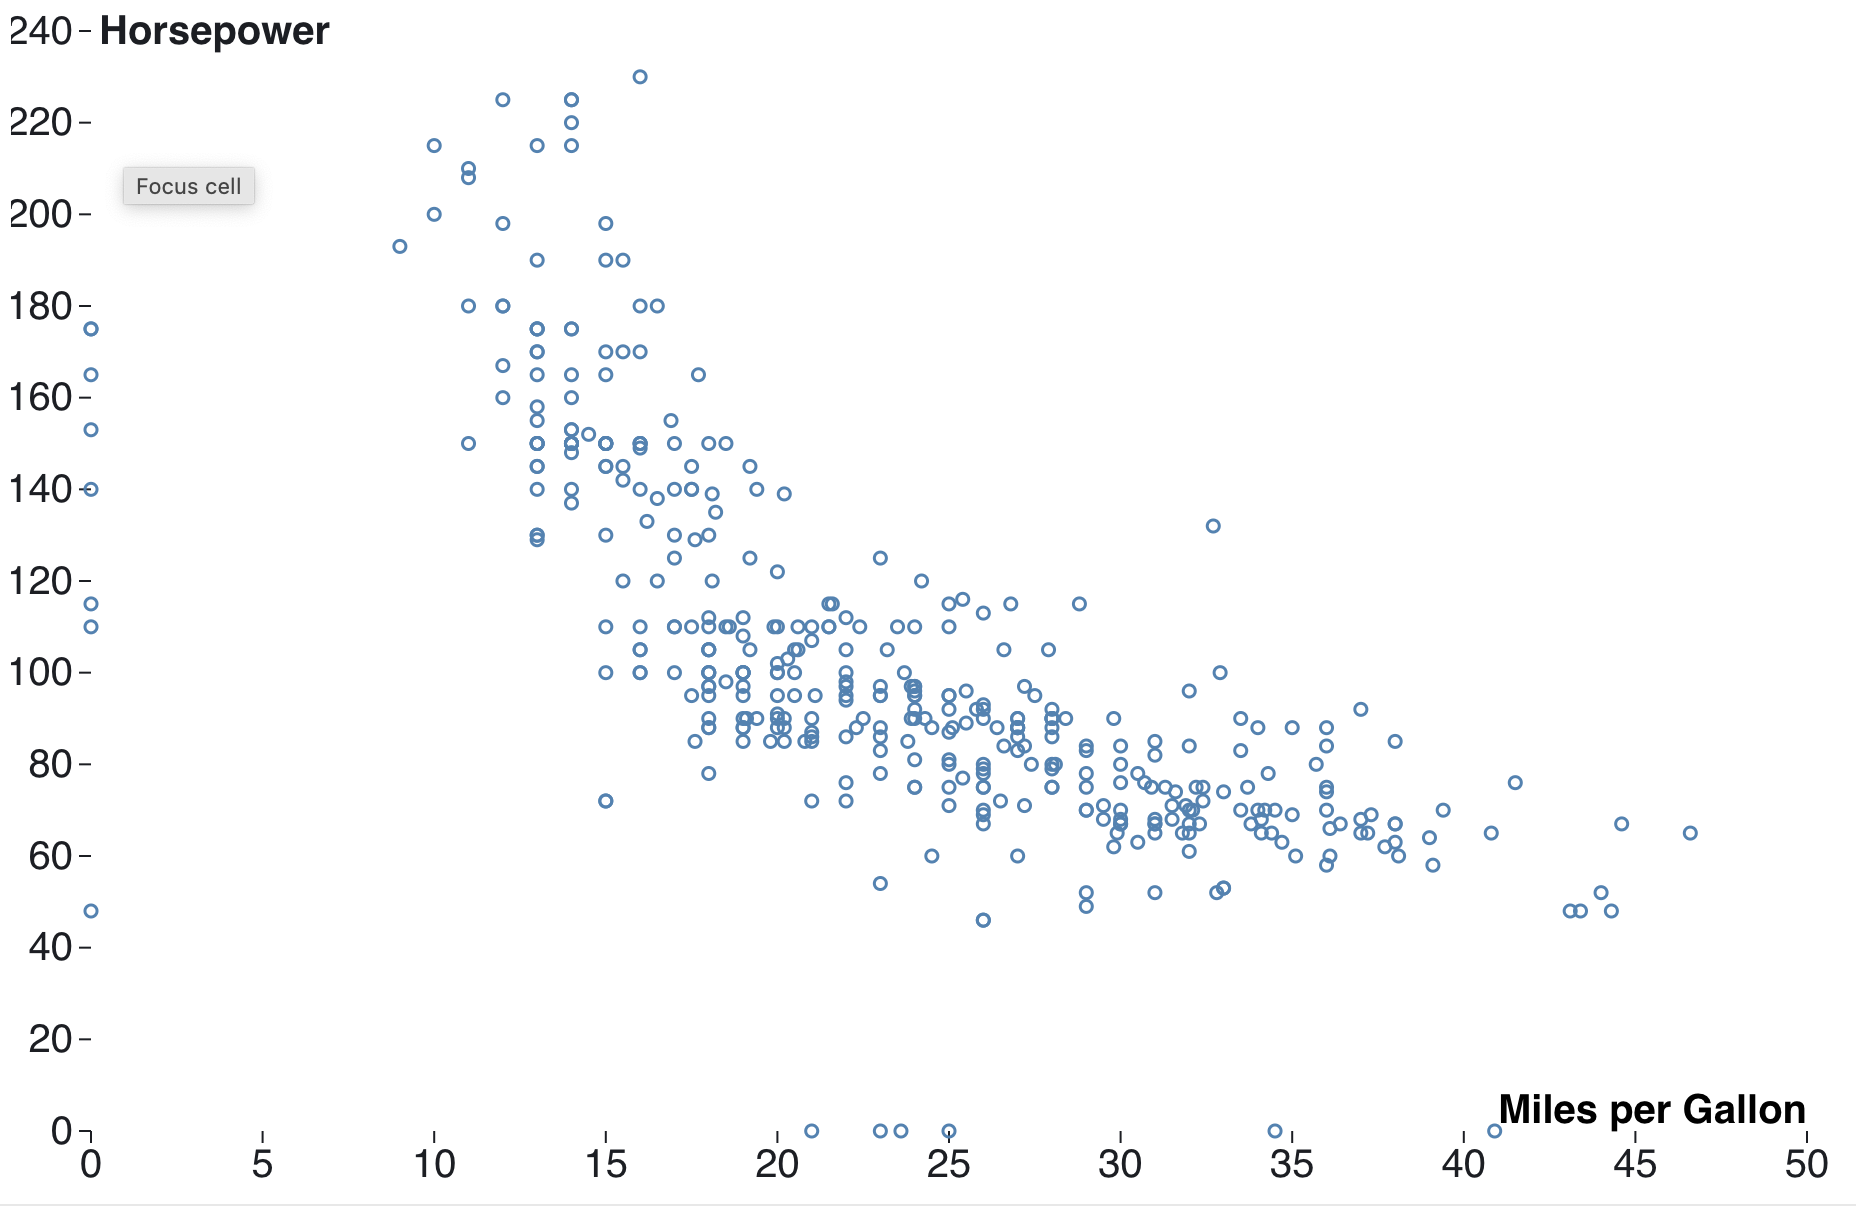
\includegraphics[width=250px]{figure/scatterplot} \end{flushleft}

\[\\[1.5cm]\]

\begin{enumerate}
\def\labelenumi{\alph{enumi}.}
\setcounter{enumi}{2}
\item
  (1 point) Imagine that the following \texttt{.attrs()} code was used
  to define the properties of each circle. Assuming your solution to
  (b), what code needs to be filled in to set the \texttt{cx} attribute?

\begin{Shaded}
\begin{Highlighting}[]
\SpecialCharTok{/}\ErrorTok{/}\NormalTok{[code defining the circles data bind]}
\FunctionTok{.attrs}\NormalTok{(\{}
\NormalTok{  cx}\SpecialCharTok{:}\NormalTok{ ... }\SpecialCharTok{/}\ErrorTok{/}\NormalTok{ fill this part }\ControlFlowTok{in}\NormalTok{,}
\NormalTok{  stroke}\SpecialCharTok{:} \StringTok{"steelblue"}\NormalTok{,}
\NormalTok{  fill}\SpecialCharTok{:} \StringTok{"none"}\NormalTok{,}
\NormalTok{  ... [assume that all other attributes have been set]}
\NormalTok{   \})}
\end{Highlighting}
\end{Shaded}
\end{enumerate}

\[\\[1.5cm]\]

\hypertarget{q5}{%
\subsubsection{Q5}\label{q5}}

This problem asks you to share your understanding of the concept of
graphical queries in data visualization.

\begin{enumerate}
\def\labelenumi{\alph{enumi}.}
\item
  (1 points) Provide a one sentence summary of the concept of graphical
  queries.

  \[\\[2.5cm]\]
\item
  (2 points) Describe an example application that uses a graphical
  query. Give details of the interactivity patterns associated with your
  example. It is enough to provide an annotated sketch.

  \[\\[2.5cm]\]
\item
  (2 point) Why is a graphical query appropriate in your example from
  part (b)? Contrast the graphical query approach with a non-graphical
  alternative.

  \[\\[2.5cm]\]
\end{enumerate}

\hypertarget{q6}{%
\subsubsection{Q6}\label{q6}}

The following code creates an interactive Shiny app that provides a
histogram that can be brushed to zoom into selected years in the
California fires dataset. A screenshot of the final visualization is
shown below. Brushing over certain years in the histogram highlights the
corresponding fires in the dotplot.

\begin{center}\includegraphics[width=400px]{figure/fires} \end{center}

\begin{enumerate}
\def\labelenumi{\alph{enumi}.}
\item
  (2 points) The starter code below sets up the overall interface, but
  doesn't support brushing. Modify the UI so that years can be brushed
  as shown in the screenshot.

\begin{Shaded}
\begin{Highlighting}[]
\NormalTok{ui }\OtherTok{\textless{}{-}} \FunctionTok{fluidPage}\NormalTok{(}
  \FunctionTok{fluidRow}\NormalTok{(}
    \FunctionTok{column}\NormalTok{(}\DecValTok{8}\NormalTok{, }\FunctionTok{plotOutput}\NormalTok{(}\StringTok{"dotplot"}\NormalTok{)),}
    \FunctionTok{column}\NormalTok{(}\DecValTok{4}\NormalTok{, }\FunctionTok{plotOutput}\NormalTok{(}\StringTok{"histogram"}\NormalTok{))}
\NormalTok{    ),}
    \FunctionTok{dataTableOutput}\NormalTok{(}\StringTok{"table"}\NormalTok{)}
\NormalTok{  )}
\end{Highlighting}
\end{Shaded}

  \[\\[1.5cm]\]
\item
  (2 points) The starter code below sets up the server. Describe how to
  modify the code so that it updates both the dotplot and the table to
  reflect the currently brushed years. Be as specific as possible. The
  second argument of \texttt{dotplot} is a vector of \texttt{TRUE} or
  \texttt{FALSE} specifying whether a given row of fires should be
  highlighted. For reference, the function is given at the end of the
  exam.

\begin{Shaded}
\begin{Highlighting}[]
\NormalTok{server }\OtherTok{\textless{}{-}} \ControlFlowTok{function}\NormalTok{(input, output) \{}
\NormalTok{  output}\SpecialCharTok{$}\NormalTok{dotplot }\OtherTok{\textless{}{-}} \FunctionTok{renderPlot}\NormalTok{(}\FunctionTok{dotplot}\NormalTok{(fires, }\CommentTok{\# ??}
\NormalTok{  output}\SpecialCharTok{$}\NormalTok{histogram }\OtherTok{\textless{}{-}} \FunctionTok{renderPlot}\NormalTok{(}\FunctionTok{year\_histogram}\NormalTok{(fires))}
\NormalTok{  output}\SpecialCharTok{$}\NormalTok{table }\OtherTok{\textless{}{-}} \FunctionTok{renderDataTable}\NormalTok{( }\CommentTok{\# ??}
\ErrorTok{\}}
\end{Highlighting}
\end{Shaded}

  \[\\[2cm]\]
\item
  (2 points) Sketch the reactivity graph of your final application. Make
  sure to distinguish input, output, and reactive nodes.

  \[\\[5cm]\]
\end{enumerate}

\hypertarget{q7}{%
\subsubsection{Q7}\label{q7}}

In this problem, we will use D3's general update pattern to visualize a
two-dimensional random walk. The result is an animation of a square that
is moving in random directions across the screen and which leaves a
``trail'' of its 20 most recently visited positions. Four screenshots
from one run of the program are given below. The first two panels were
taken within the first few timesteps, which is why they show less than
20 squares.

\includegraphics[width=100px]{figure/rw1}
\includegraphics[width=100px]{figure/rw2}
\includegraphics[width=100px]{figure/rw3}
\includegraphics[width=100px]{figure/rw4}

You have been given the starter code below.
\texttt{update\_walk\_data()} pushes an array element specifying the
next location of the random walk. It also removes any array elements
from more than 20 time units in the past. The \texttt{x} and \texttt{y}
attributes within each element give the \texttt{x} and \texttt{y}
coordinates of the walk. \texttt{timepoint} specifies the time step at
which the array element was added. The definition of
\texttt{update\_walk\_data()} is given at the end of this exam for
reference.

\begin{Shaded}
\begin{Highlighting}[]
\NormalTok{let walk }\OtherTok{=}\NormalTok{ [\{x}\SpecialCharTok{:} \DecValTok{250}\NormalTok{, y}\SpecialCharTok{:} \DecValTok{250}\NormalTok{, timepoint}\SpecialCharTok{:} \DecValTok{0}\NormalTok{\}],}
\NormalTok{  timepoint }\OtherTok{=} \DecValTok{0}\NormalTok{;}

\ControlFlowTok{function} \FunctionTok{update}\NormalTok{() \{}
\NormalTok{  timepoint }\SpecialCharTok{+}\ErrorTok{=} \DecValTok{1}\NormalTok{;}
\NormalTok{  walk }\OtherTok{=} \FunctionTok{update\_walk\_data}\NormalTok{(walk, timepoint)}

\NormalTok{  let rw }\OtherTok{=} \FunctionTok{d3.select}\NormalTok{(}\StringTok{"svg"}\NormalTok{)}
    \FunctionTok{.selectAll}\NormalTok{(}\StringTok{"rect"}\NormalTok{)}
    \FunctionTok{.data}\NormalTok{(walk, }\AttributeTok{d =}\SpecialCharTok{\textgreater{}}\NormalTok{ d.timepoint)}
\NormalTok{\}}

\FunctionTok{d3.interval}\NormalTok{(update, }\DecValTok{100}\NormalTok{)}
\end{Highlighting}
\end{Shaded}

\begin{enumerate}
\def\labelenumi{\alph{enumi}.}
\tightlist
\item
  (2 points) How would you modify the \texttt{update()} function so that
  it removes all ``old'' random walk locations that are no longer
  contained within the \texttt{walk} array?
\end{enumerate}

\[\\[2.5cm]\]

\begin{enumerate}
\def\labelenumi{\alph{enumi}.}
\setcounter{enumi}{1}
\tightlist
\item
  (2 points) How would you modify the \texttt{update()} function so
  that, after each time step, it appends a rectangle at the newest
  random walk location?
\end{enumerate}

\[\\[2.5cm]\]

\begin{enumerate}
\def\labelenumi{\alph{enumi}.}
\setcounter{enumi}{2}
\tightlist
\item
  (2 points) Notice that in the screenshots above, the random walk
  squares become fainter the more time units they are into the past. How
  would you modify the \texttt{update()} function to reflect this?
\end{enumerate}

\[\\[2.5cm]\]

\hypertarget{code-supplement}{%
\subsubsection{Code Supplement}\label{code-supplement}}

\emph{Supplementary code for Q6}

\begin{Shaded}
\begin{Highlighting}[]
\NormalTok{dotplot }\OtherTok{\textless{}{-}} \ControlFlowTok{function}\NormalTok{(df, selected) \{}
\NormalTok{  df }\SpecialCharTok{\%\textgreater{}\%}
    \FunctionTok{mutate}\NormalTok{(}
      \AttributeTok{selected =}\NormalTok{ selected,}
      \AttributeTok{selected =} \FunctionTok{factor}\NormalTok{(selected, }\AttributeTok{levels =} \FunctionTok{c}\NormalTok{(}\StringTok{"TRUE"}\NormalTok{, }\StringTok{"FALSE"}\NormalTok{))}
\NormalTok{      ) }\SpecialCharTok{\%\textgreater{}\%}
  \FunctionTok{ggplot}\NormalTok{() }\SpecialCharTok{+}
    \FunctionTok{geom\_point}\NormalTok{(}\FunctionTok{aes}\NormalTok{(day\_of\_year, Counties, }\AttributeTok{size =}\NormalTok{ AcresBurned, }\AttributeTok{col =}\NormalTok{ selected)) }\SpecialCharTok{+}
    \FunctionTok{scale\_color\_manual}\NormalTok{(}\AttributeTok{values =} \FunctionTok{c}\NormalTok{(}\StringTok{"orange"}\NormalTok{, }\StringTok{"\#e3e3e3"}\NormalTok{))}
\NormalTok{\}}
  
\NormalTok{year\_histogram }\OtherTok{\textless{}{-}} \ControlFlowTok{function}\NormalTok{(fires) \{}
  \FunctionTok{ggplot}\NormalTok{(fires) }\SpecialCharTok{+}
    \FunctionTok{geom\_histogram}\NormalTok{(}\FunctionTok{aes}\NormalTok{(year))}
\NormalTok{\}}
\end{Highlighting}
\end{Shaded}

\emph{Supplementary code for Q7}

\begin{Shaded}
\begin{Highlighting}[]
\NormalTok{let  generator }\OtherTok{=} \FunctionTok{d3.randomUniform}\NormalTok{(}\SpecialCharTok{{-}}\DecValTok{10}\NormalTok{, }\DecValTok{10}\NormalTok{);}

\ControlFlowTok{function} \FunctionTok{update\_walk\_data}\NormalTok{(walk, timepoint) \{}
  \FunctionTok{walk.push}\NormalTok{(\{}
\NormalTok{    x}\SpecialCharTok{:}\NormalTok{ walk[walk.length }\SpecialCharTok{{-}} \DecValTok{1}\NormalTok{].x }\SpecialCharTok{+} \FunctionTok{generator}\NormalTok{(),}
\NormalTok{    y}\SpecialCharTok{:}\NormalTok{ walk[walk.length }\SpecialCharTok{{-}} \DecValTok{1}\NormalTok{].y }\SpecialCharTok{+} \FunctionTok{generator}\NormalTok{(),}
\NormalTok{    timepoint}\SpecialCharTok{:}\NormalTok{ timepoint}
\NormalTok{  \})}
\NormalTok{  return }\FunctionTok{walk.filter}\NormalTok{(}\AttributeTok{d =}\SpecialCharTok{\textgreater{}}\NormalTok{ d.timepoint }\SpecialCharTok{\textgreater{}}\NormalTok{ timepoint }\SpecialCharTok{{-}} \DecValTok{20}\NormalTok{)}
\NormalTok{\}}
\end{Highlighting}
\end{Shaded}


\end{document}
